\documentclass[..\main.tex]{subfile}
\begin{document}
\subsection{Results}
We sart with the simplest system, a superconductor involving some vertical periodic boundary conditions.
We use an attractive potential of $U=-2$ for the on site superconductivity in the superconductor and zero ervywhere else.
\begin{figure}[H]
  \centering
  % GNUPLOT: LaTeX picture with Postscript
\begingroup
  % Encoding inside the plot.  In the header of your document, this encoding
  % should to defined, e.g., by using
  % \usepackage[cp1252,<other encodings>]{inputenc}
  \inputencoding{cp1252}%
  \makeatletter
  \providecommand\color[2][]{%
    \GenericError{(gnuplot) \space\space\space\@spaces}{%
      Package color not loaded in conjunction with
      terminal option `colourtext'%
    }{See the gnuplot documentation for explanation.%
    }{Either use 'blacktext' in gnuplot or load the package
      color.sty in LaTeX.}%
    \renewcommand\color[2][]{}%
  }%
  \providecommand\includegraphics[2][]{%
    \GenericError{(gnuplot) \space\space\space\@spaces}{%
      Package graphicx or graphics not loaded%
    }{See the gnuplot documentation for explanation.%
    }{The gnuplot epslatex terminal needs graphicx.sty or graphics.sty.}%
    \renewcommand\includegraphics[2][]{}%
  }%
  \providecommand\rotatebox[2]{#2}%
  \@ifundefined{ifGPcolor}{%
    \newif\ifGPcolor
    \GPcolortrue
  }{}%
  \@ifundefined{ifGPblacktext}{%
    \newif\ifGPblacktext
    \GPblacktextfalse
  }{}%
  % define a \g@addto@macro without @ in the name:
  \let\gplgaddtomacro\g@addto@macro
  % define empty templates for all commands taking text:
  \gdef\gplbacktext{}%
  \gdef\gplfronttext{}%
  \makeatother
  \ifGPblacktext
    % no textcolor at all
    \def\colorrgb#1{}%
    \def\colorgray#1{}%
  \else
    % gray or color?
    \ifGPcolor
      \def\colorrgb#1{\color[rgb]{#1}}%
      \def\colorgray#1{\color[gray]{#1}}%
      \expandafter\def\csname LTw\endcsname{\color{white}}%
      \expandafter\def\csname LTb\endcsname{\color{black}}%
      \expandafter\def\csname LTa\endcsname{\color{black}}%
      \expandafter\def\csname LT0\endcsname{\color[rgb]{1,0,0}}%
      \expandafter\def\csname LT1\endcsname{\color[rgb]{0,1,0}}%
      \expandafter\def\csname LT2\endcsname{\color[rgb]{0,0,1}}%
      \expandafter\def\csname LT3\endcsname{\color[rgb]{1,0,1}}%
      \expandafter\def\csname LT4\endcsname{\color[rgb]{0,1,1}}%
      \expandafter\def\csname LT5\endcsname{\color[rgb]{1,1,0}}%
      \expandafter\def\csname LT6\endcsname{\color[rgb]{0,0,0}}%
      \expandafter\def\csname LT7\endcsname{\color[rgb]{1,0.3,0}}%
      \expandafter\def\csname LT8\endcsname{\color[rgb]{0.5,0.5,0.5}}%
    \else
      % gray
      \def\colorrgb#1{\color{black}}%
      \def\colorgray#1{\color[gray]{#1}}%
      \expandafter\def\csname LTw\endcsname{\color{white}}%
      \expandafter\def\csname LTb\endcsname{\color{black}}%
      \expandafter\def\csname LTa\endcsname{\color{black}}%
      \expandafter\def\csname LT0\endcsname{\color{black}}%
      \expandafter\def\csname LT1\endcsname{\color{black}}%
      \expandafter\def\csname LT2\endcsname{\color{black}}%
      \expandafter\def\csname LT3\endcsname{\color{black}}%
      \expandafter\def\csname LT4\endcsname{\color{black}}%
      \expandafter\def\csname LT5\endcsname{\color{black}}%
      \expandafter\def\csname LT6\endcsname{\color{black}}%
      \expandafter\def\csname LT7\endcsname{\color{black}}%
      \expandafter\def\csname LT8\endcsname{\color{black}}%
    \fi
  \fi
    \setlength{\unitlength}{0.0500bp}%
    \ifx\gptboxheight\undefined%
      \newlength{\gptboxheight}%
      \newlength{\gptboxwidth}%
      \newsavebox{\gptboxtext}%
    \fi%
    \setlength{\fboxrule}{0.5pt}%
    \setlength{\fboxsep}{1pt}%
    \definecolor{tbcol}{rgb}{1,1,1}%
\begin{picture}(5760.00,3772.00)%
    \gplgaddtomacro\gplbacktext{%
      \csname LTb\endcsname%%
      \put(1807,3313){\makebox(0,0){\strut{}SC}}%
      \put(3953,3313){\makebox(0,0){\strut{}AM}}%
    }%
    \gplgaddtomacro\gplfronttext{%
      \csname LTb\endcsname%%
      \put(1073,742){\makebox(0,0){\scriptsize 2}}%
      \put(1525,742){\makebox(0,0){\scriptsize 4}}%
      \put(1977,742){\makebox(0,0){\scriptsize 6}}%
      \put(2429,742){\makebox(0,0){\scriptsize 8}}%
      \put(2880,742){\makebox(0,0){\scriptsize 10}}%
      \put(3331,742){\makebox(0,0){\scriptsize 12}}%
      \put(3783,742){\makebox(0,0){\scriptsize 14}}%
      \put(4235,742){\makebox(0,0){\scriptsize 16}}%
      \put(4687,742){\makebox(0,0){\scriptsize 18}}%
      \put(2880,478){\makebox(0,0){\small\textbf{Lattice site $i_x$ in $\bm{e}_x$}}}%
      \put(480,1006){\makebox(0,0){\scriptsize 2}}%
      \put(480,1254){\makebox(0,0){\scriptsize 4}}%
      \put(480,1501){\makebox(0,0){\scriptsize 6}}%
      \put(480,1749){\makebox(0,0){\scriptsize 8}}%
      \put(480,1996){\makebox(0,0){\scriptsize 10}}%
      \put(480,2243){\makebox(0,0){\scriptsize 12}}%
      \put(480,2491){\makebox(0,0){\scriptsize 14}}%
      \put(480,2738){\makebox(0,0){\scriptsize 16}}%
      \put(480,2986){\makebox(0,0){\scriptsize 18}}%
      \put(150,1996){\rotatebox{-270.00}{\makebox(0,0){\small\textbf{Lattice site $i_y$ in $\bm{e}_y$}}}}%
      \put(5743,820){\makebox(0,0){\tiny \(0\)}}%
      \put(5743,1212){\makebox(0,0){\tiny \(1e{-06}\)}}%
      \put(5743,1604){\makebox(0,0){\tiny \(2e{-06}\)}}%
      \put(5743,1996){\makebox(0,0){\tiny \(3e{-06}\)}}%
      \put(5743,2388){\makebox(0,0){\tiny \(4e{-06}\)}}%
      \put(5743,2780){\makebox(0,0){\tiny \(5e{-06}\)}}%
      \put(5743,3171){\makebox(0,0){\tiny \(6e{-06}\)}}%
    }%
    \gplbacktext
    \put(0,0){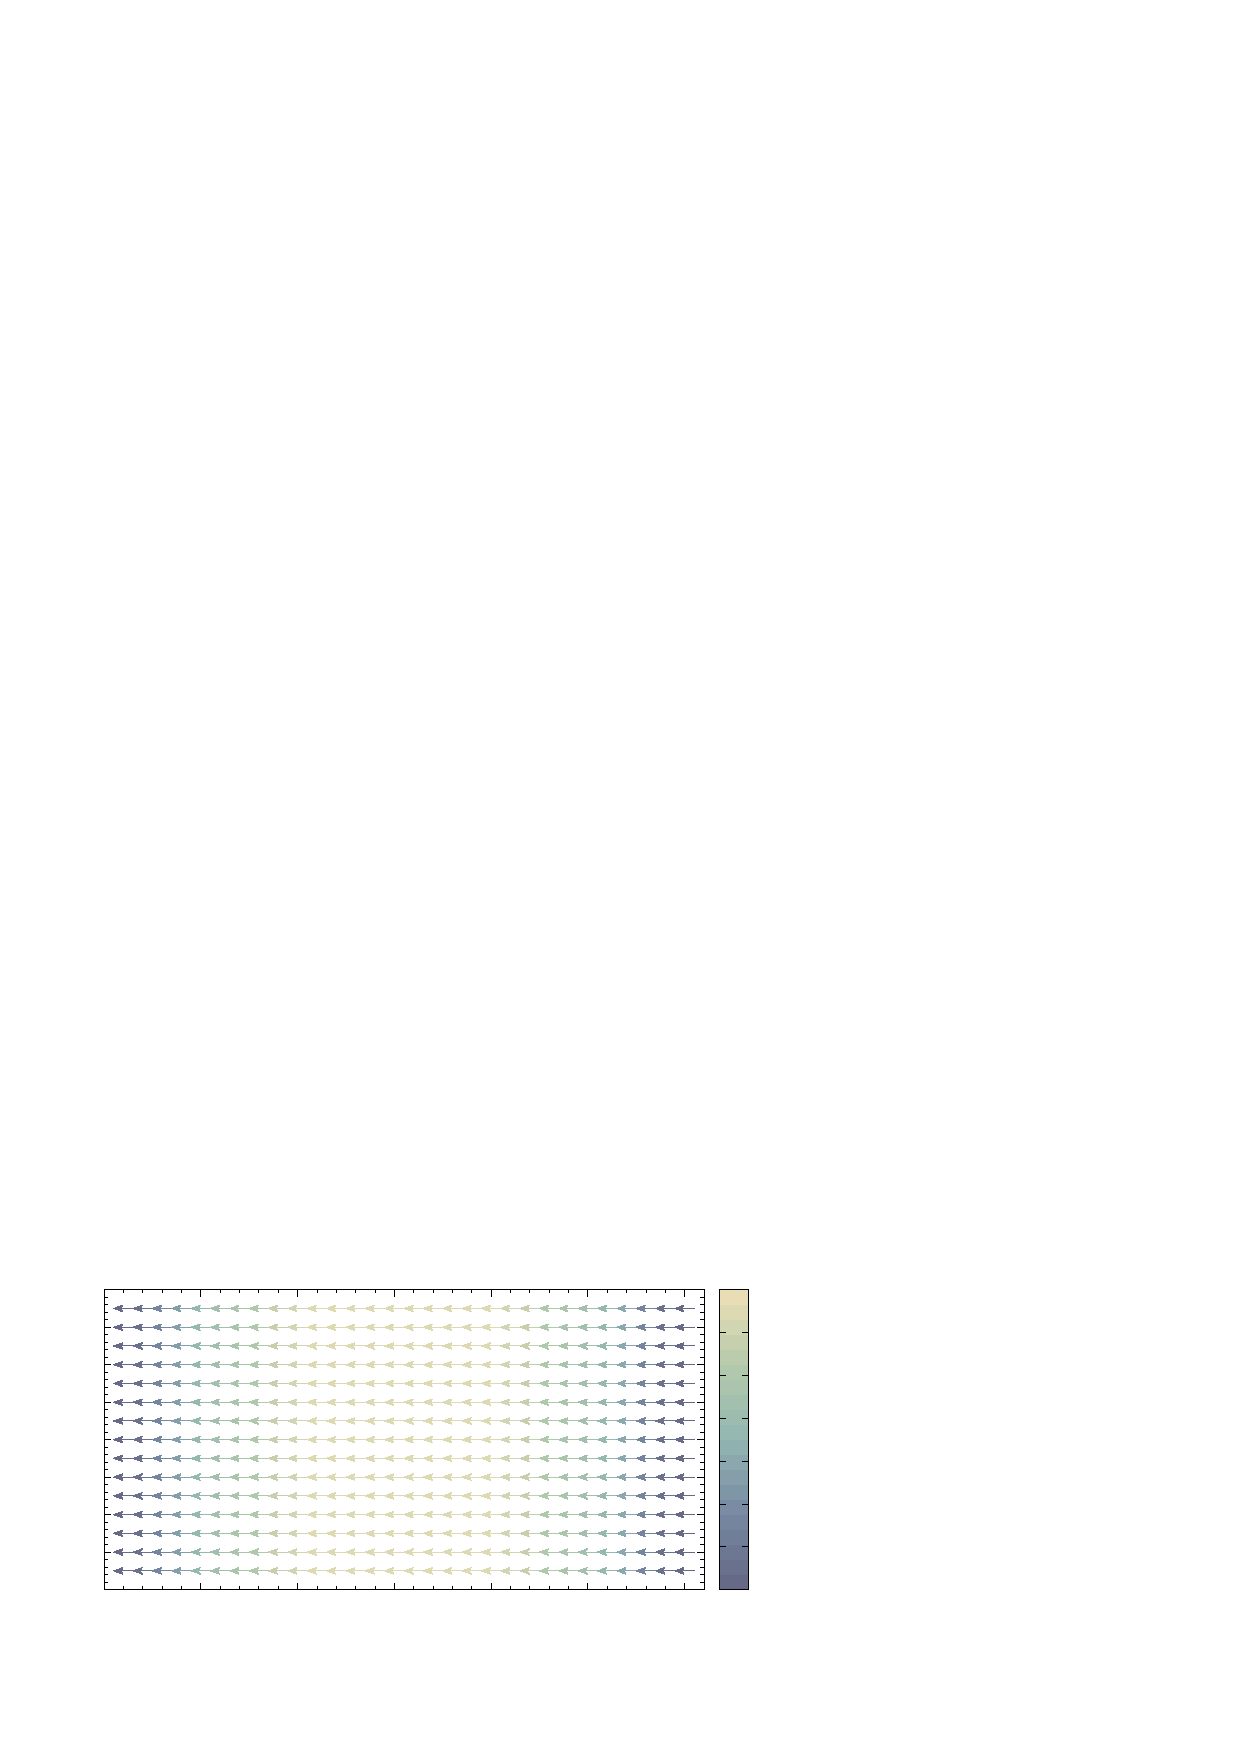
\includegraphics[width={288.00bp},height={188.60bp}]{Plots/SC10AM10/HeatMap/VertHorizBC/plot}}%
    \gplfronttext
  \end{picture}%
\endgroup


  \caption{The expectation value of the c operators taking part into the gap as $\Delta_i = U_i\langle c_{i\uparrow}c_{i\downarrow}\rangle$. The  
  vertical periodic boundary condition makes each site on the same $x$-coordinate having the same value.
    We can then make an average on each of these collumns and polt the result.}
\end{figure}
The superconducting gap lays arround $0.01\cdot U$ and $0.16\cdot U$ \rem{eV?} for the range of selected chemical potential. Further we observe a 
clear symmetry in the Cooper pairs distribution arround the level $\mu =0$. The overlapp of the Fermi surface with the s-wave seams
to be the same for $\pm\mu$. Further we observe some oscillations on the left and right sides. On these locations the sites have only three
neigbhours, there are open boundaries, the rest is vaccum. One can see this lack of neigbhours as  impurties in the system. 
These oszillations may be caused by Andrev bound states \cite{Bobkov_2024}, that may form because the quasiparticles are reflected at the boundary.
These can interfer with the Cooper pairs and cause the oscillations in the spacial representation of the energy gap.\\

From this we can complexify the system by adding a different material on the right side of the superconductor. 
The most simple one is a normal metal (N) that has a hopping $t$ of $1$ in every direction.
Then we can repalce it with an alternating hopping $t+m$ depending on a $\uparrow\uparrow$ interaction
and a $t-m$ depending on a $\downarrow\downarrow$ interaction. This is a ferromagnetic material (FM).
Making the sign of $m$ alternating if we have an interaction along the $x$ or the $y$ axis describes an altermagnet (AM).
Here we set $m=0.5$ and study different results for the chemical potential $\mu<0$ and compare the AM
with the others. $\ast$ represent a placeholder for the material a curve describes.\\
\begin{figure}[H]
  \centering
  % GNUPLOT: LaTeX picture with Postscript
\begingroup
  % Encoding inside the plot.  In the header of your document, this encoding
  % should to defined, e.g., by using
  % \usepackage[cp1252,<other encodings>]{inputenc}
  \inputencoding{cp1252}%
  \makeatletter
  \providecommand\color[2][]{%
    \GenericError{(gnuplot) \space\space\space\@spaces}{%
      Package color not loaded in conjunction with
      terminal option `colourtext'%
    }{See the gnuplot documentation for explanation.%
    }{Either use 'blacktext' in gnuplot or load the package
      color.sty in LaTeX.}%
    \renewcommand\color[2][]{}%
  }%
  \providecommand\includegraphics[2][]{%
    \GenericError{(gnuplot) \space\space\space\@spaces}{%
      Package graphicx or graphics not loaded%
    }{See the gnuplot documentation for explanation.%
    }{The gnuplot epslatex terminal needs graphicx.sty or graphics.sty.}%
    \renewcommand\includegraphics[2][]{}%
  }%
  \providecommand\rotatebox[2]{#2}%
  \@ifundefined{ifGPcolor}{%
    \newif\ifGPcolor
    \GPcolortrue
  }{}%
  \@ifundefined{ifGPblacktext}{%
    \newif\ifGPblacktext
    \GPblacktextfalse
  }{}%
  % define a \g@addto@macro without @ in the name:
  \let\gplgaddtomacro\g@addto@macro
  % define empty templates for all commands taking text:
  \gdef\gplbacktext{}%
  \gdef\gplfronttext{}%
  \makeatother
  \ifGPblacktext
    % no textcolor at all
    \def\colorrgb#1{}%
    \def\colorgray#1{}%
  \else
    % gray or color?
    \ifGPcolor
      \def\colorrgb#1{\color[rgb]{#1}}%
      \def\colorgray#1{\color[gray]{#1}}%
      \expandafter\def\csname LTw\endcsname{\color{white}}%
      \expandafter\def\csname LTb\endcsname{\color{black}}%
      \expandafter\def\csname LTa\endcsname{\color{black}}%
      \expandafter\def\csname LT0\endcsname{\color[rgb]{1,0,0}}%
      \expandafter\def\csname LT1\endcsname{\color[rgb]{0,1,0}}%
      \expandafter\def\csname LT2\endcsname{\color[rgb]{0,0,1}}%
      \expandafter\def\csname LT3\endcsname{\color[rgb]{1,0,1}}%
      \expandafter\def\csname LT4\endcsname{\color[rgb]{0,1,1}}%
      \expandafter\def\csname LT5\endcsname{\color[rgb]{1,1,0}}%
      \expandafter\def\csname LT6\endcsname{\color[rgb]{0,0,0}}%
      \expandafter\def\csname LT7\endcsname{\color[rgb]{1,0.3,0}}%
      \expandafter\def\csname LT8\endcsname{\color[rgb]{0.5,0.5,0.5}}%
    \else
      % gray
      \def\colorrgb#1{\color{black}}%
      \def\colorgray#1{\color[gray]{#1}}%
      \expandafter\def\csname LTw\endcsname{\color{white}}%
      \expandafter\def\csname LTb\endcsname{\color{black}}%
      \expandafter\def\csname LTa\endcsname{\color{black}}%
      \expandafter\def\csname LT0\endcsname{\color{black}}%
      \expandafter\def\csname LT1\endcsname{\color{black}}%
      \expandafter\def\csname LT2\endcsname{\color{black}}%
      \expandafter\def\csname LT3\endcsname{\color{black}}%
      \expandafter\def\csname LT4\endcsname{\color{black}}%
      \expandafter\def\csname LT5\endcsname{\color{black}}%
      \expandafter\def\csname LT6\endcsname{\color{black}}%
      \expandafter\def\csname LT7\endcsname{\color{black}}%
      \expandafter\def\csname LT8\endcsname{\color{black}}%
    \fi
  \fi
    \setlength{\unitlength}{0.0500bp}%
    \ifx\gptboxheight\undefined%
      \newlength{\gptboxheight}%
      \newlength{\gptboxwidth}%
      \newsavebox{\gptboxtext}%
    \fi%
    \setlength{\fboxrule}{0.5pt}%
    \setlength{\fboxsep}{1pt}%
    \definecolor{tbcol}{rgb}{1,1,1}%
\begin{picture}(5760.00,3772.00)%
    \gplgaddtomacro\gplbacktext{%
      \csname LTb\endcsname%%
      \put(1807,3313){\makebox(0,0){\strut{}SC}}%
      \put(3953,3313){\makebox(0,0){\strut{}AM}}%
    }%
    \gplgaddtomacro\gplfronttext{%
      \csname LTb\endcsname%%
      \put(1073,742){\makebox(0,0){\scriptsize 2}}%
      \put(1525,742){\makebox(0,0){\scriptsize 4}}%
      \put(1977,742){\makebox(0,0){\scriptsize 6}}%
      \put(2429,742){\makebox(0,0){\scriptsize 8}}%
      \put(2880,742){\makebox(0,0){\scriptsize 10}}%
      \put(3331,742){\makebox(0,0){\scriptsize 12}}%
      \put(3783,742){\makebox(0,0){\scriptsize 14}}%
      \put(4235,742){\makebox(0,0){\scriptsize 16}}%
      \put(4687,742){\makebox(0,0){\scriptsize 18}}%
      \put(2880,478){\makebox(0,0){\small\textbf{Lattice site $i_x$ in $\bm{e}_x$}}}%
      \put(480,1006){\makebox(0,0){\scriptsize 2}}%
      \put(480,1254){\makebox(0,0){\scriptsize 4}}%
      \put(480,1501){\makebox(0,0){\scriptsize 6}}%
      \put(480,1749){\makebox(0,0){\scriptsize 8}}%
      \put(480,1996){\makebox(0,0){\scriptsize 10}}%
      \put(480,2243){\makebox(0,0){\scriptsize 12}}%
      \put(480,2491){\makebox(0,0){\scriptsize 14}}%
      \put(480,2738){\makebox(0,0){\scriptsize 16}}%
      \put(480,2986){\makebox(0,0){\scriptsize 18}}%
      \put(150,1996){\rotatebox{-270.00}{\makebox(0,0){\small\textbf{Lattice site $i_y$ in $\bm{e}_y$}}}}%
      \put(5743,820){\makebox(0,0){\tiny \(0\)}}%
      \put(5743,1212){\makebox(0,0){\tiny \(1e{-06}\)}}%
      \put(5743,1604){\makebox(0,0){\tiny \(2e{-06}\)}}%
      \put(5743,1996){\makebox(0,0){\tiny \(3e{-06}\)}}%
      \put(5743,2388){\makebox(0,0){\tiny \(4e{-06}\)}}%
      \put(5743,2780){\makebox(0,0){\tiny \(5e{-06}\)}}%
      \put(5743,3171){\makebox(0,0){\tiny \(6e{-06}\)}}%
    }%
    \gplbacktext
    \put(0,0){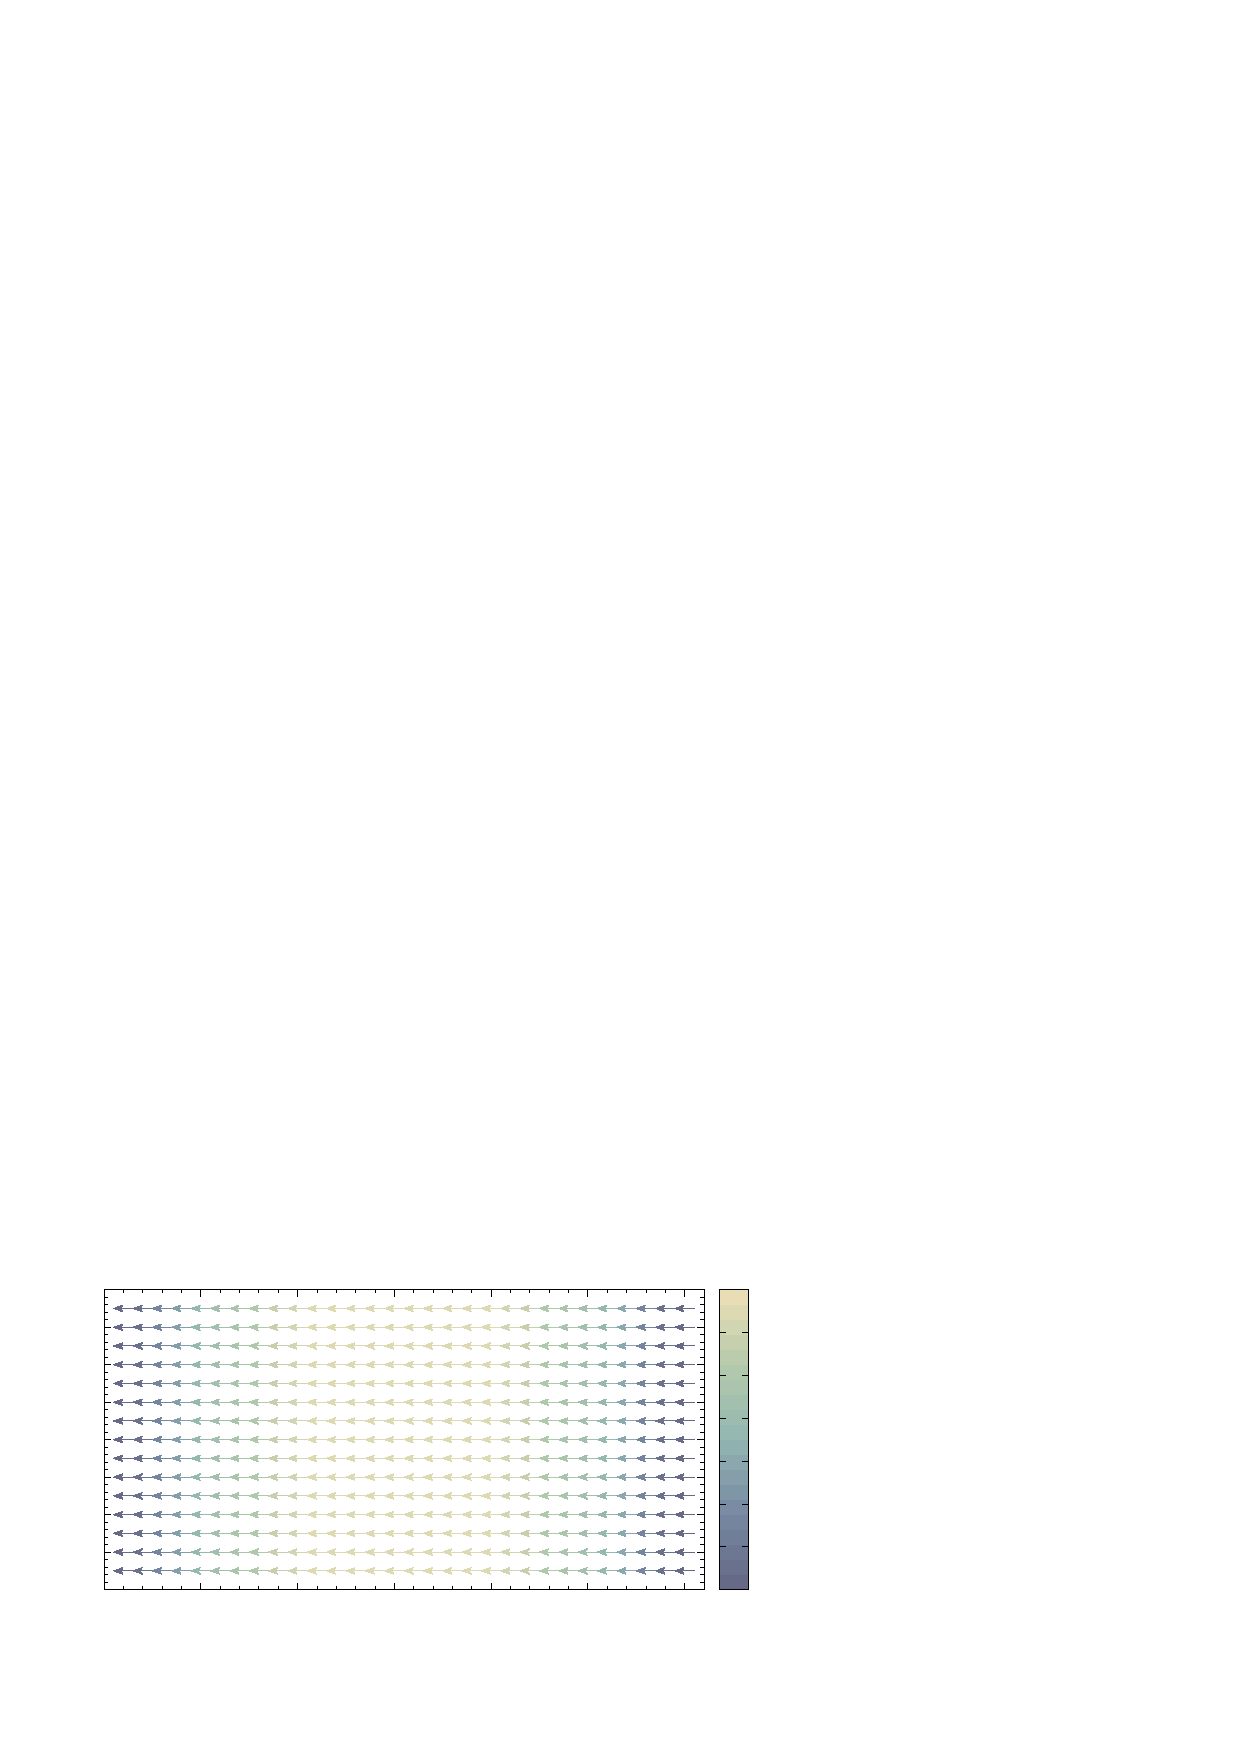
\includegraphics[width={288.00bp},height={188.60bp}]{Plots/SC10AM10/HeatMap/VertHorizBC/plot}}%
    \gplfronttext
  \end{picture}%
\endgroup


  \caption{Evolution of the gap in the $x$ direction for a junction of SC-N SC-FM and SC-AM at $\mu=-0.5$.}
\end{figure}\begin{figure}[H]
  \centering
  % GNUPLOT: LaTeX picture with Postscript
\begingroup
  % Encoding inside the plot.  In the header of your document, this encoding
  % should to defined, e.g., by using
  % \usepackage[cp1252,<other encodings>]{inputenc}
  \inputencoding{cp1252}%
  \makeatletter
  \providecommand\color[2][]{%
    \GenericError{(gnuplot) \space\space\space\@spaces}{%
      Package color not loaded in conjunction with
      terminal option `colourtext'%
    }{See the gnuplot documentation for explanation.%
    }{Either use 'blacktext' in gnuplot or load the package
      color.sty in LaTeX.}%
    \renewcommand\color[2][]{}%
  }%
  \providecommand\includegraphics[2][]{%
    \GenericError{(gnuplot) \space\space\space\@spaces}{%
      Package graphicx or graphics not loaded%
    }{See the gnuplot documentation for explanation.%
    }{The gnuplot epslatex terminal needs graphicx.sty or graphics.sty.}%
    \renewcommand\includegraphics[2][]{}%
  }%
  \providecommand\rotatebox[2]{#2}%
  \@ifundefined{ifGPcolor}{%
    \newif\ifGPcolor
    \GPcolortrue
  }{}%
  \@ifundefined{ifGPblacktext}{%
    \newif\ifGPblacktext
    \GPblacktextfalse
  }{}%
  % define a \g@addto@macro without @ in the name:
  \let\gplgaddtomacro\g@addto@macro
  % define empty templates for all commands taking text:
  \gdef\gplbacktext{}%
  \gdef\gplfronttext{}%
  \makeatother
  \ifGPblacktext
    % no textcolor at all
    \def\colorrgb#1{}%
    \def\colorgray#1{}%
  \else
    % gray or color?
    \ifGPcolor
      \def\colorrgb#1{\color[rgb]{#1}}%
      \def\colorgray#1{\color[gray]{#1}}%
      \expandafter\def\csname LTw\endcsname{\color{white}}%
      \expandafter\def\csname LTb\endcsname{\color{black}}%
      \expandafter\def\csname LTa\endcsname{\color{black}}%
      \expandafter\def\csname LT0\endcsname{\color[rgb]{1,0,0}}%
      \expandafter\def\csname LT1\endcsname{\color[rgb]{0,1,0}}%
      \expandafter\def\csname LT2\endcsname{\color[rgb]{0,0,1}}%
      \expandafter\def\csname LT3\endcsname{\color[rgb]{1,0,1}}%
      \expandafter\def\csname LT4\endcsname{\color[rgb]{0,1,1}}%
      \expandafter\def\csname LT5\endcsname{\color[rgb]{1,1,0}}%
      \expandafter\def\csname LT6\endcsname{\color[rgb]{0,0,0}}%
      \expandafter\def\csname LT7\endcsname{\color[rgb]{1,0.3,0}}%
      \expandafter\def\csname LT8\endcsname{\color[rgb]{0.5,0.5,0.5}}%
    \else
      % gray
      \def\colorrgb#1{\color{black}}%
      \def\colorgray#1{\color[gray]{#1}}%
      \expandafter\def\csname LTw\endcsname{\color{white}}%
      \expandafter\def\csname LTb\endcsname{\color{black}}%
      \expandafter\def\csname LTa\endcsname{\color{black}}%
      \expandafter\def\csname LT0\endcsname{\color{black}}%
      \expandafter\def\csname LT1\endcsname{\color{black}}%
      \expandafter\def\csname LT2\endcsname{\color{black}}%
      \expandafter\def\csname LT3\endcsname{\color{black}}%
      \expandafter\def\csname LT4\endcsname{\color{black}}%
      \expandafter\def\csname LT5\endcsname{\color{black}}%
      \expandafter\def\csname LT6\endcsname{\color{black}}%
      \expandafter\def\csname LT7\endcsname{\color{black}}%
      \expandafter\def\csname LT8\endcsname{\color{black}}%
    \fi
  \fi
    \setlength{\unitlength}{0.0500bp}%
    \ifx\gptboxheight\undefined%
      \newlength{\gptboxheight}%
      \newlength{\gptboxwidth}%
      \newsavebox{\gptboxtext}%
    \fi%
    \setlength{\fboxrule}{0.5pt}%
    \setlength{\fboxsep}{1pt}%
    \definecolor{tbcol}{rgb}{1,1,1}%
\begin{picture}(5760.00,3772.00)%
    \gplgaddtomacro\gplbacktext{%
      \csname LTb\endcsname%%
      \put(1807,3313){\makebox(0,0){\strut{}SC}}%
      \put(3953,3313){\makebox(0,0){\strut{}AM}}%
    }%
    \gplgaddtomacro\gplfronttext{%
      \csname LTb\endcsname%%
      \put(1073,742){\makebox(0,0){\scriptsize 2}}%
      \put(1525,742){\makebox(0,0){\scriptsize 4}}%
      \put(1977,742){\makebox(0,0){\scriptsize 6}}%
      \put(2429,742){\makebox(0,0){\scriptsize 8}}%
      \put(2880,742){\makebox(0,0){\scriptsize 10}}%
      \put(3331,742){\makebox(0,0){\scriptsize 12}}%
      \put(3783,742){\makebox(0,0){\scriptsize 14}}%
      \put(4235,742){\makebox(0,0){\scriptsize 16}}%
      \put(4687,742){\makebox(0,0){\scriptsize 18}}%
      \put(2880,478){\makebox(0,0){\small\textbf{Lattice site $i_x$ in $\bm{e}_x$}}}%
      \put(480,1006){\makebox(0,0){\scriptsize 2}}%
      \put(480,1254){\makebox(0,0){\scriptsize 4}}%
      \put(480,1501){\makebox(0,0){\scriptsize 6}}%
      \put(480,1749){\makebox(0,0){\scriptsize 8}}%
      \put(480,1996){\makebox(0,0){\scriptsize 10}}%
      \put(480,2243){\makebox(0,0){\scriptsize 12}}%
      \put(480,2491){\makebox(0,0){\scriptsize 14}}%
      \put(480,2738){\makebox(0,0){\scriptsize 16}}%
      \put(480,2986){\makebox(0,0){\scriptsize 18}}%
      \put(150,1996){\rotatebox{-270.00}{\makebox(0,0){\small\textbf{Lattice site $i_y$ in $\bm{e}_y$}}}}%
      \put(5743,820){\makebox(0,0){\tiny \(0\)}}%
      \put(5743,1212){\makebox(0,0){\tiny \(1e{-06}\)}}%
      \put(5743,1604){\makebox(0,0){\tiny \(2e{-06}\)}}%
      \put(5743,1996){\makebox(0,0){\tiny \(3e{-06}\)}}%
      \put(5743,2388){\makebox(0,0){\tiny \(4e{-06}\)}}%
      \put(5743,2780){\makebox(0,0){\tiny \(5e{-06}\)}}%
      \put(5743,3171){\makebox(0,0){\tiny \(6e{-06}\)}}%
    }%
    \gplbacktext
    \put(0,0){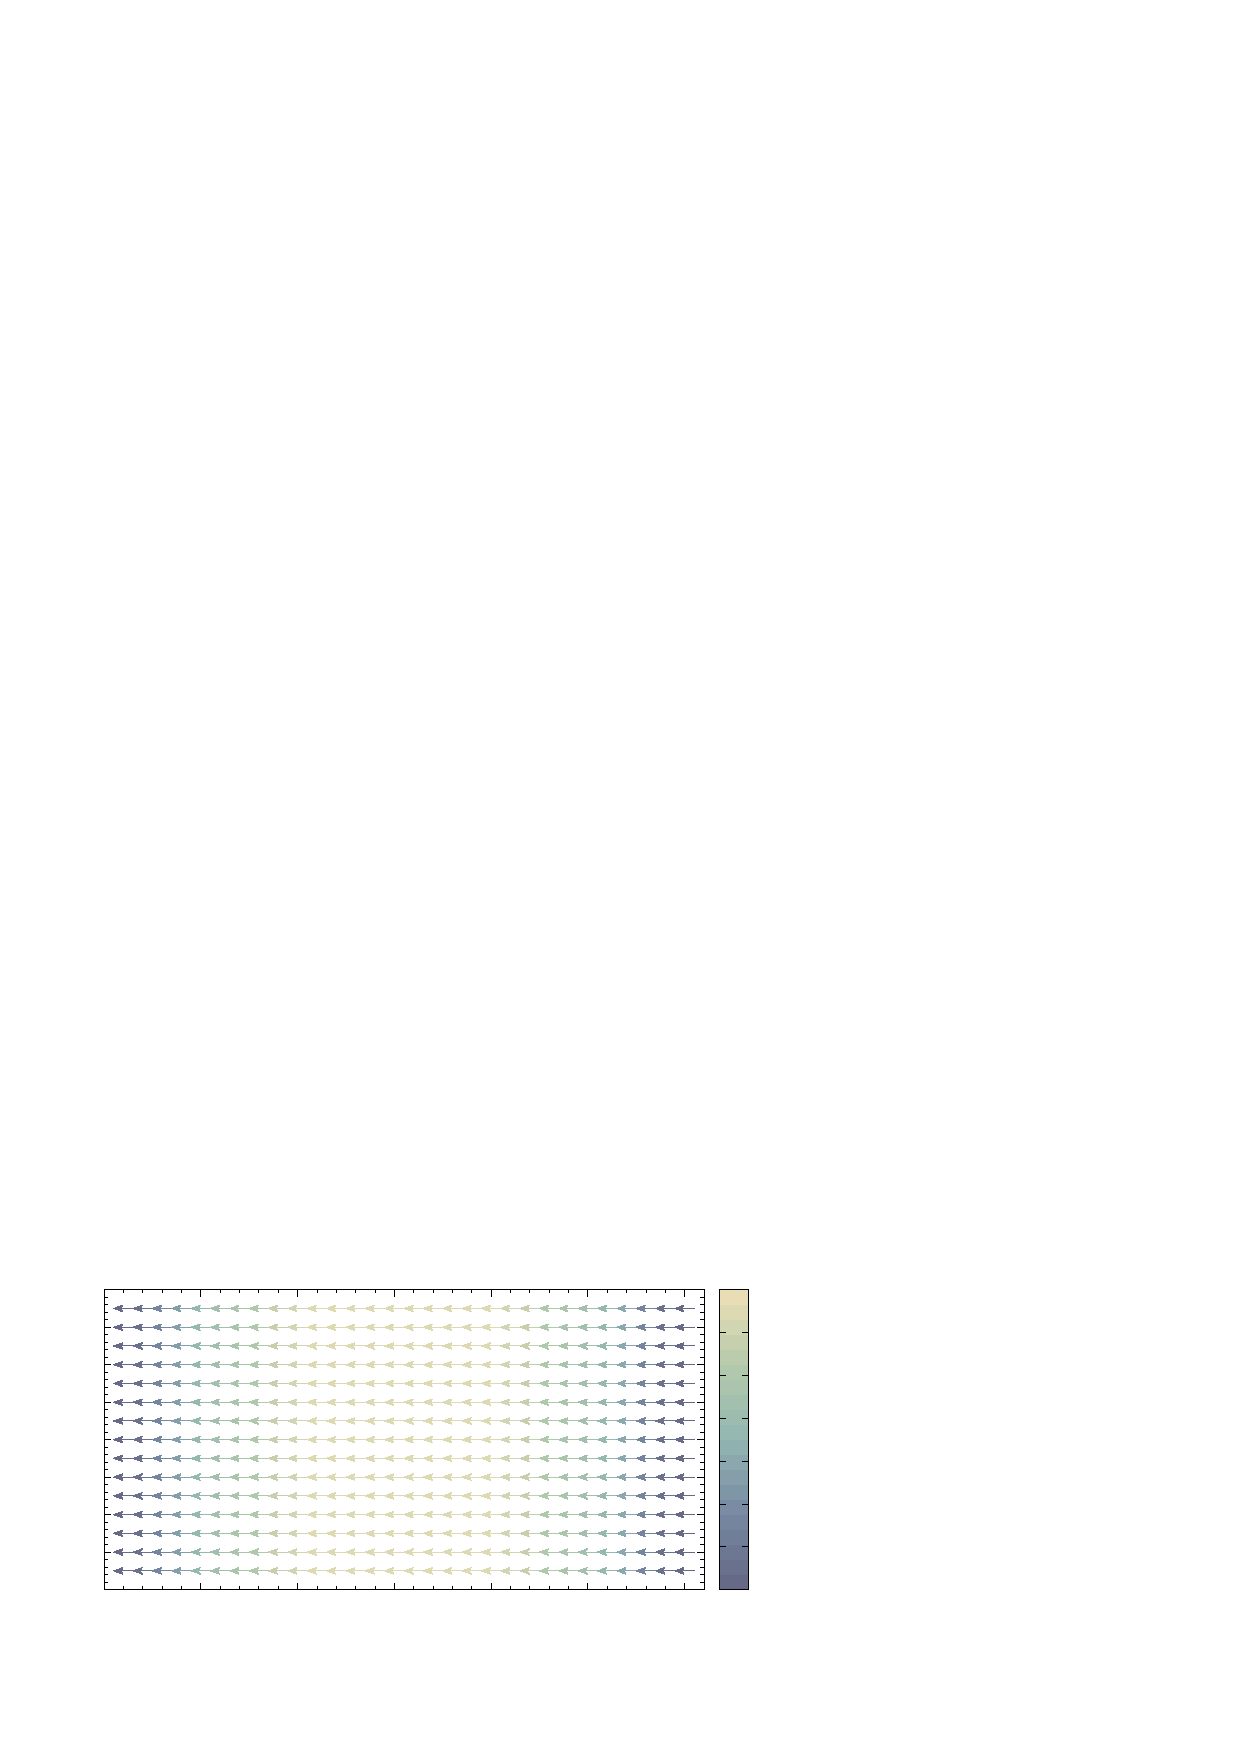
\includegraphics[width={288.00bp},height={188.60bp}]{Plots/SC10AM10/HeatMap/VertHorizBC/plot}}%
    \gplfronttext
  \end{picture}%
\endgroup


  \caption{Evolution of the gap in the $x$ direction for a junction of SC-N SC-FM and SC-AM at $\mu=-1.5$.}
\end{figure}
\begin{figure}[H]
  \centering
  % GNUPLOT: LaTeX picture with Postscript
\begingroup
  % Encoding inside the plot.  In the header of your document, this encoding
  % should to defined, e.g., by using
  % \usepackage[cp1252,<other encodings>]{inputenc}
  \inputencoding{cp1252}%
  \makeatletter
  \providecommand\color[2][]{%
    \GenericError{(gnuplot) \space\space\space\@spaces}{%
      Package color not loaded in conjunction with
      terminal option `colourtext'%
    }{See the gnuplot documentation for explanation.%
    }{Either use 'blacktext' in gnuplot or load the package
      color.sty in LaTeX.}%
    \renewcommand\color[2][]{}%
  }%
  \providecommand\includegraphics[2][]{%
    \GenericError{(gnuplot) \space\space\space\@spaces}{%
      Package graphicx or graphics not loaded%
    }{See the gnuplot documentation for explanation.%
    }{The gnuplot epslatex terminal needs graphicx.sty or graphics.sty.}%
    \renewcommand\includegraphics[2][]{}%
  }%
  \providecommand\rotatebox[2]{#2}%
  \@ifundefined{ifGPcolor}{%
    \newif\ifGPcolor
    \GPcolortrue
  }{}%
  \@ifundefined{ifGPblacktext}{%
    \newif\ifGPblacktext
    \GPblacktextfalse
  }{}%
  % define a \g@addto@macro without @ in the name:
  \let\gplgaddtomacro\g@addto@macro
  % define empty templates for all commands taking text:
  \gdef\gplbacktext{}%
  \gdef\gplfronttext{}%
  \makeatother
  \ifGPblacktext
    % no textcolor at all
    \def\colorrgb#1{}%
    \def\colorgray#1{}%
  \else
    % gray or color?
    \ifGPcolor
      \def\colorrgb#1{\color[rgb]{#1}}%
      \def\colorgray#1{\color[gray]{#1}}%
      \expandafter\def\csname LTw\endcsname{\color{white}}%
      \expandafter\def\csname LTb\endcsname{\color{black}}%
      \expandafter\def\csname LTa\endcsname{\color{black}}%
      \expandafter\def\csname LT0\endcsname{\color[rgb]{1,0,0}}%
      \expandafter\def\csname LT1\endcsname{\color[rgb]{0,1,0}}%
      \expandafter\def\csname LT2\endcsname{\color[rgb]{0,0,1}}%
      \expandafter\def\csname LT3\endcsname{\color[rgb]{1,0,1}}%
      \expandafter\def\csname LT4\endcsname{\color[rgb]{0,1,1}}%
      \expandafter\def\csname LT5\endcsname{\color[rgb]{1,1,0}}%
      \expandafter\def\csname LT6\endcsname{\color[rgb]{0,0,0}}%
      \expandafter\def\csname LT7\endcsname{\color[rgb]{1,0.3,0}}%
      \expandafter\def\csname LT8\endcsname{\color[rgb]{0.5,0.5,0.5}}%
    \else
      % gray
      \def\colorrgb#1{\color{black}}%
      \def\colorgray#1{\color[gray]{#1}}%
      \expandafter\def\csname LTw\endcsname{\color{white}}%
      \expandafter\def\csname LTb\endcsname{\color{black}}%
      \expandafter\def\csname LTa\endcsname{\color{black}}%
      \expandafter\def\csname LT0\endcsname{\color{black}}%
      \expandafter\def\csname LT1\endcsname{\color{black}}%
      \expandafter\def\csname LT2\endcsname{\color{black}}%
      \expandafter\def\csname LT3\endcsname{\color{black}}%
      \expandafter\def\csname LT4\endcsname{\color{black}}%
      \expandafter\def\csname LT5\endcsname{\color{black}}%
      \expandafter\def\csname LT6\endcsname{\color{black}}%
      \expandafter\def\csname LT7\endcsname{\color{black}}%
      \expandafter\def\csname LT8\endcsname{\color{black}}%
    \fi
  \fi
    \setlength{\unitlength}{0.0500bp}%
    \ifx\gptboxheight\undefined%
      \newlength{\gptboxheight}%
      \newlength{\gptboxwidth}%
      \newsavebox{\gptboxtext}%
    \fi%
    \setlength{\fboxrule}{0.5pt}%
    \setlength{\fboxsep}{1pt}%
    \definecolor{tbcol}{rgb}{1,1,1}%
\begin{picture}(5760.00,3772.00)%
    \gplgaddtomacro\gplbacktext{%
      \csname LTb\endcsname%%
      \put(1807,3313){\makebox(0,0){\strut{}SC}}%
      \put(3953,3313){\makebox(0,0){\strut{}AM}}%
    }%
    \gplgaddtomacro\gplfronttext{%
      \csname LTb\endcsname%%
      \put(1073,742){\makebox(0,0){\scriptsize 2}}%
      \put(1525,742){\makebox(0,0){\scriptsize 4}}%
      \put(1977,742){\makebox(0,0){\scriptsize 6}}%
      \put(2429,742){\makebox(0,0){\scriptsize 8}}%
      \put(2880,742){\makebox(0,0){\scriptsize 10}}%
      \put(3331,742){\makebox(0,0){\scriptsize 12}}%
      \put(3783,742){\makebox(0,0){\scriptsize 14}}%
      \put(4235,742){\makebox(0,0){\scriptsize 16}}%
      \put(4687,742){\makebox(0,0){\scriptsize 18}}%
      \put(2880,478){\makebox(0,0){\small\textbf{Lattice site $i_x$ in $\bm{e}_x$}}}%
      \put(480,1006){\makebox(0,0){\scriptsize 2}}%
      \put(480,1254){\makebox(0,0){\scriptsize 4}}%
      \put(480,1501){\makebox(0,0){\scriptsize 6}}%
      \put(480,1749){\makebox(0,0){\scriptsize 8}}%
      \put(480,1996){\makebox(0,0){\scriptsize 10}}%
      \put(480,2243){\makebox(0,0){\scriptsize 12}}%
      \put(480,2491){\makebox(0,0){\scriptsize 14}}%
      \put(480,2738){\makebox(0,0){\scriptsize 16}}%
      \put(480,2986){\makebox(0,0){\scriptsize 18}}%
      \put(150,1996){\rotatebox{-270.00}{\makebox(0,0){\small\textbf{Lattice site $i_y$ in $\bm{e}_y$}}}}%
      \put(5743,820){\makebox(0,0){\tiny \(0\)}}%
      \put(5743,1212){\makebox(0,0){\tiny \(1e{-06}\)}}%
      \put(5743,1604){\makebox(0,0){\tiny \(2e{-06}\)}}%
      \put(5743,1996){\makebox(0,0){\tiny \(3e{-06}\)}}%
      \put(5743,2388){\makebox(0,0){\tiny \(4e{-06}\)}}%
      \put(5743,2780){\makebox(0,0){\tiny \(5e{-06}\)}}%
      \put(5743,3171){\makebox(0,0){\tiny \(6e{-06}\)}}%
    }%
    \gplbacktext
    \put(0,0){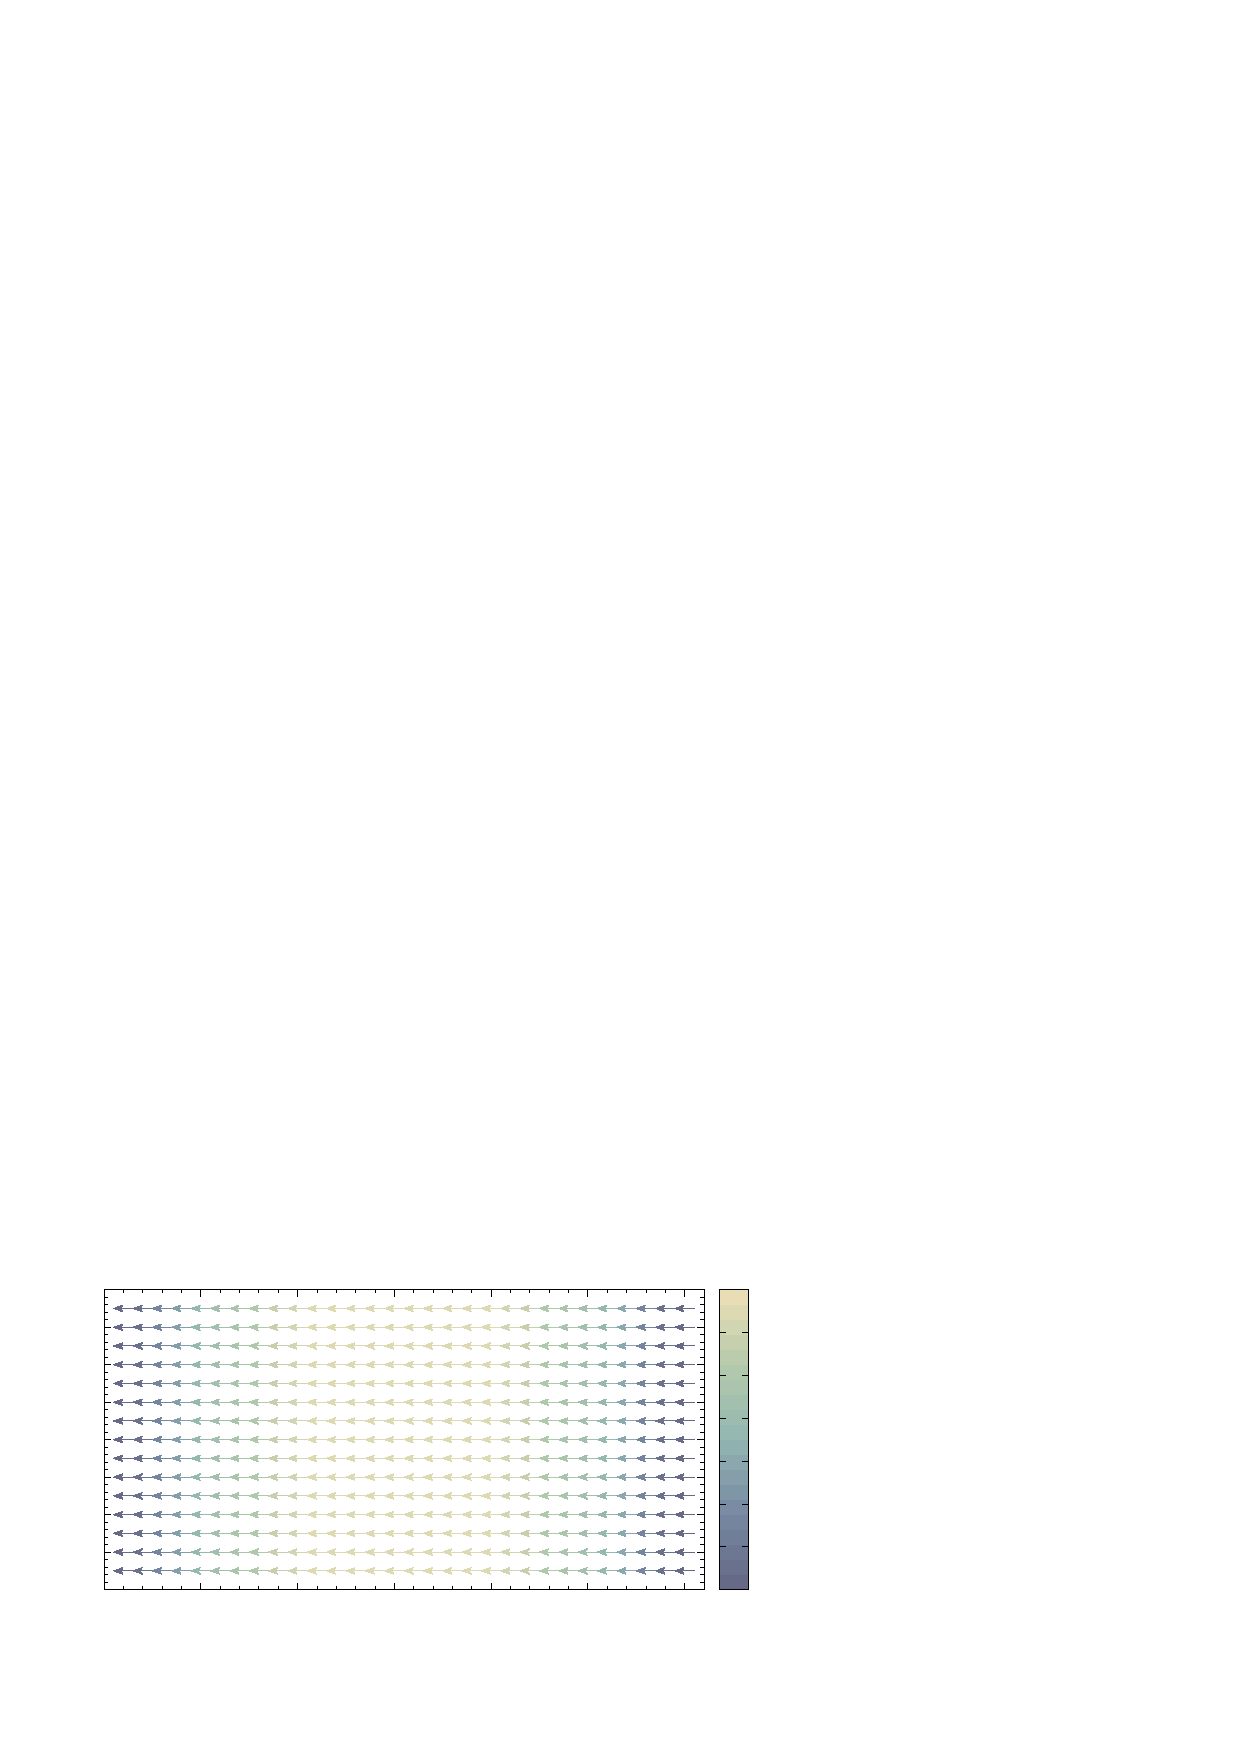
\includegraphics[width={288.00bp},height={188.60bp}]{Plots/SC10AM10/HeatMap/VertHorizBC/plot}}%
    \gplfronttext
  \end{picture}%
\endgroup


  \caption{Evolution of the gap in the $x$ direction for a junction of SC-N SC-FM and SC-AM at $\mu=-2.5$.}
\end{figure}
We first take a look at the superconductor (SC). Inside of it the gap seams not to be affected by the chemical potential
and sattels arround $0.1\cdot U$. 
We can compare to the normal metal case. We have a clear decay of the gap after entering the normal metal (N). At this point 
study that were alreay made tend to have an exponential decay of the gap \cite{Mjos2019}. Having a logarithmic scale we would
exepect a more straight line but this is still a reasonable exponential decay. A way to approch the line would be to increase the 
resolution of the lattice, as well as simulating a more squared one. This decay makes the expectation value having an order of 
magnetude of difference from one side to the other of the N. For the smallest $\mu$ we have  


Further we see that both the FM and the AM add some oscilations in the decay. \\

The ferromagnet seams to following closely the normal metal for $\mu=-0.5,-1.5$. It is intersting to note a realy nice exponential
decay when having a chemical potential of $-2.5$ modulated by oscillations. For the AM the initial decay is stronger in the sites near the 
interface than in the FM. Then the decay seams to follow the FM. We observe about the same number of oscilaltions in the FM and the AM.
For $\mu=-0.5$ we observe a clean line in the first four sites of the AM. Than we have oscilaltions and the Cooper-pairs are more present
than expected regarding the initial decay. The reason might be that the first oscillation combined with the inital decay make the line
reach it's second deepest point (arround $10^{-4}$) and looks therfore very small compared to the rest.

The oscillation amplitude seams to have increased as well,
we observe nearly two orders of magnetude in their amplitude
 
 The maximal
 oscsillation amplitude seams to be the same in every context with a value arround an order of magnetude.



We now simualte how does the s-wave superconductivity behave on a diagonal interface. We focus on three different values of $\mu<0$.  
\begin{figure}[H]
    \centering
    % GNUPLOT: LaTeX picture with Postscript
\begingroup
  % Encoding inside the plot.  In the header of your document, this encoding
  % should to defined, e.g., by using
  % \usepackage[cp1252,<other encodings>]{inputenc}
  \inputencoding{cp1252}%
  \makeatletter
  \providecommand\color[2][]{%
    \GenericError{(gnuplot) \space\space\space\@spaces}{%
      Package color not loaded in conjunction with
      terminal option `colourtext'%
    }{See the gnuplot documentation for explanation.%
    }{Either use 'blacktext' in gnuplot or load the package
      color.sty in LaTeX.}%
    \renewcommand\color[2][]{}%
  }%
  \providecommand\includegraphics[2][]{%
    \GenericError{(gnuplot) \space\space\space\@spaces}{%
      Package graphicx or graphics not loaded%
    }{See the gnuplot documentation for explanation.%
    }{The gnuplot epslatex terminal needs graphicx.sty or graphics.sty.}%
    \renewcommand\includegraphics[2][]{}%
  }%
  \providecommand\rotatebox[2]{#2}%
  \@ifundefined{ifGPcolor}{%
    \newif\ifGPcolor
    \GPcolortrue
  }{}%
  \@ifundefined{ifGPblacktext}{%
    \newif\ifGPblacktext
    \GPblacktextfalse
  }{}%
  % define a \g@addto@macro without @ in the name:
  \let\gplgaddtomacro\g@addto@macro
  % define empty templates for all commands taking text:
  \gdef\gplbacktext{}%
  \gdef\gplfronttext{}%
  \makeatother
  \ifGPblacktext
    % no textcolor at all
    \def\colorrgb#1{}%
    \def\colorgray#1{}%
  \else
    % gray or color?
    \ifGPcolor
      \def\colorrgb#1{\color[rgb]{#1}}%
      \def\colorgray#1{\color[gray]{#1}}%
      \expandafter\def\csname LTw\endcsname{\color{white}}%
      \expandafter\def\csname LTb\endcsname{\color{black}}%
      \expandafter\def\csname LTa\endcsname{\color{black}}%
      \expandafter\def\csname LT0\endcsname{\color[rgb]{1,0,0}}%
      \expandafter\def\csname LT1\endcsname{\color[rgb]{0,1,0}}%
      \expandafter\def\csname LT2\endcsname{\color[rgb]{0,0,1}}%
      \expandafter\def\csname LT3\endcsname{\color[rgb]{1,0,1}}%
      \expandafter\def\csname LT4\endcsname{\color[rgb]{0,1,1}}%
      \expandafter\def\csname LT5\endcsname{\color[rgb]{1,1,0}}%
      \expandafter\def\csname LT6\endcsname{\color[rgb]{0,0,0}}%
      \expandafter\def\csname LT7\endcsname{\color[rgb]{1,0.3,0}}%
      \expandafter\def\csname LT8\endcsname{\color[rgb]{0.5,0.5,0.5}}%
    \else
      % gray
      \def\colorrgb#1{\color{black}}%
      \def\colorgray#1{\color[gray]{#1}}%
      \expandafter\def\csname LTw\endcsname{\color{white}}%
      \expandafter\def\csname LTb\endcsname{\color{black}}%
      \expandafter\def\csname LTa\endcsname{\color{black}}%
      \expandafter\def\csname LT0\endcsname{\color{black}}%
      \expandafter\def\csname LT1\endcsname{\color{black}}%
      \expandafter\def\csname LT2\endcsname{\color{black}}%
      \expandafter\def\csname LT3\endcsname{\color{black}}%
      \expandafter\def\csname LT4\endcsname{\color{black}}%
      \expandafter\def\csname LT5\endcsname{\color{black}}%
      \expandafter\def\csname LT6\endcsname{\color{black}}%
      \expandafter\def\csname LT7\endcsname{\color{black}}%
      \expandafter\def\csname LT8\endcsname{\color{black}}%
    \fi
  \fi
    \setlength{\unitlength}{0.0500bp}%
    \ifx\gptboxheight\undefined%
      \newlength{\gptboxheight}%
      \newlength{\gptboxwidth}%
      \newsavebox{\gptboxtext}%
    \fi%
    \setlength{\fboxrule}{0.5pt}%
    \setlength{\fboxsep}{1pt}%
    \definecolor{tbcol}{rgb}{1,1,1}%
\begin{picture}(5760.00,3772.00)%
    \gplgaddtomacro\gplbacktext{%
      \csname LTb\endcsname%%
      \put(1807,3313){\makebox(0,0){\strut{}SC}}%
      \put(3953,3313){\makebox(0,0){\strut{}AM}}%
    }%
    \gplgaddtomacro\gplfronttext{%
      \csname LTb\endcsname%%
      \put(1073,742){\makebox(0,0){\scriptsize 2}}%
      \put(1525,742){\makebox(0,0){\scriptsize 4}}%
      \put(1977,742){\makebox(0,0){\scriptsize 6}}%
      \put(2429,742){\makebox(0,0){\scriptsize 8}}%
      \put(2880,742){\makebox(0,0){\scriptsize 10}}%
      \put(3331,742){\makebox(0,0){\scriptsize 12}}%
      \put(3783,742){\makebox(0,0){\scriptsize 14}}%
      \put(4235,742){\makebox(0,0){\scriptsize 16}}%
      \put(4687,742){\makebox(0,0){\scriptsize 18}}%
      \put(2880,478){\makebox(0,0){\small\textbf{Lattice site $i_x$ in $\bm{e}_x$}}}%
      \put(480,1006){\makebox(0,0){\scriptsize 2}}%
      \put(480,1254){\makebox(0,0){\scriptsize 4}}%
      \put(480,1501){\makebox(0,0){\scriptsize 6}}%
      \put(480,1749){\makebox(0,0){\scriptsize 8}}%
      \put(480,1996){\makebox(0,0){\scriptsize 10}}%
      \put(480,2243){\makebox(0,0){\scriptsize 12}}%
      \put(480,2491){\makebox(0,0){\scriptsize 14}}%
      \put(480,2738){\makebox(0,0){\scriptsize 16}}%
      \put(480,2986){\makebox(0,0){\scriptsize 18}}%
      \put(150,1996){\rotatebox{-270.00}{\makebox(0,0){\small\textbf{Lattice site $i_y$ in $\bm{e}_y$}}}}%
      \put(5743,820){\makebox(0,0){\tiny \(0\)}}%
      \put(5743,1212){\makebox(0,0){\tiny \(1e{-06}\)}}%
      \put(5743,1604){\makebox(0,0){\tiny \(2e{-06}\)}}%
      \put(5743,1996){\makebox(0,0){\tiny \(3e{-06}\)}}%
      \put(5743,2388){\makebox(0,0){\tiny \(4e{-06}\)}}%
      \put(5743,2780){\makebox(0,0){\tiny \(5e{-06}\)}}%
      \put(5743,3171){\makebox(0,0){\tiny \(6e{-06}\)}}%
    }%
    \gplbacktext
    \put(0,0){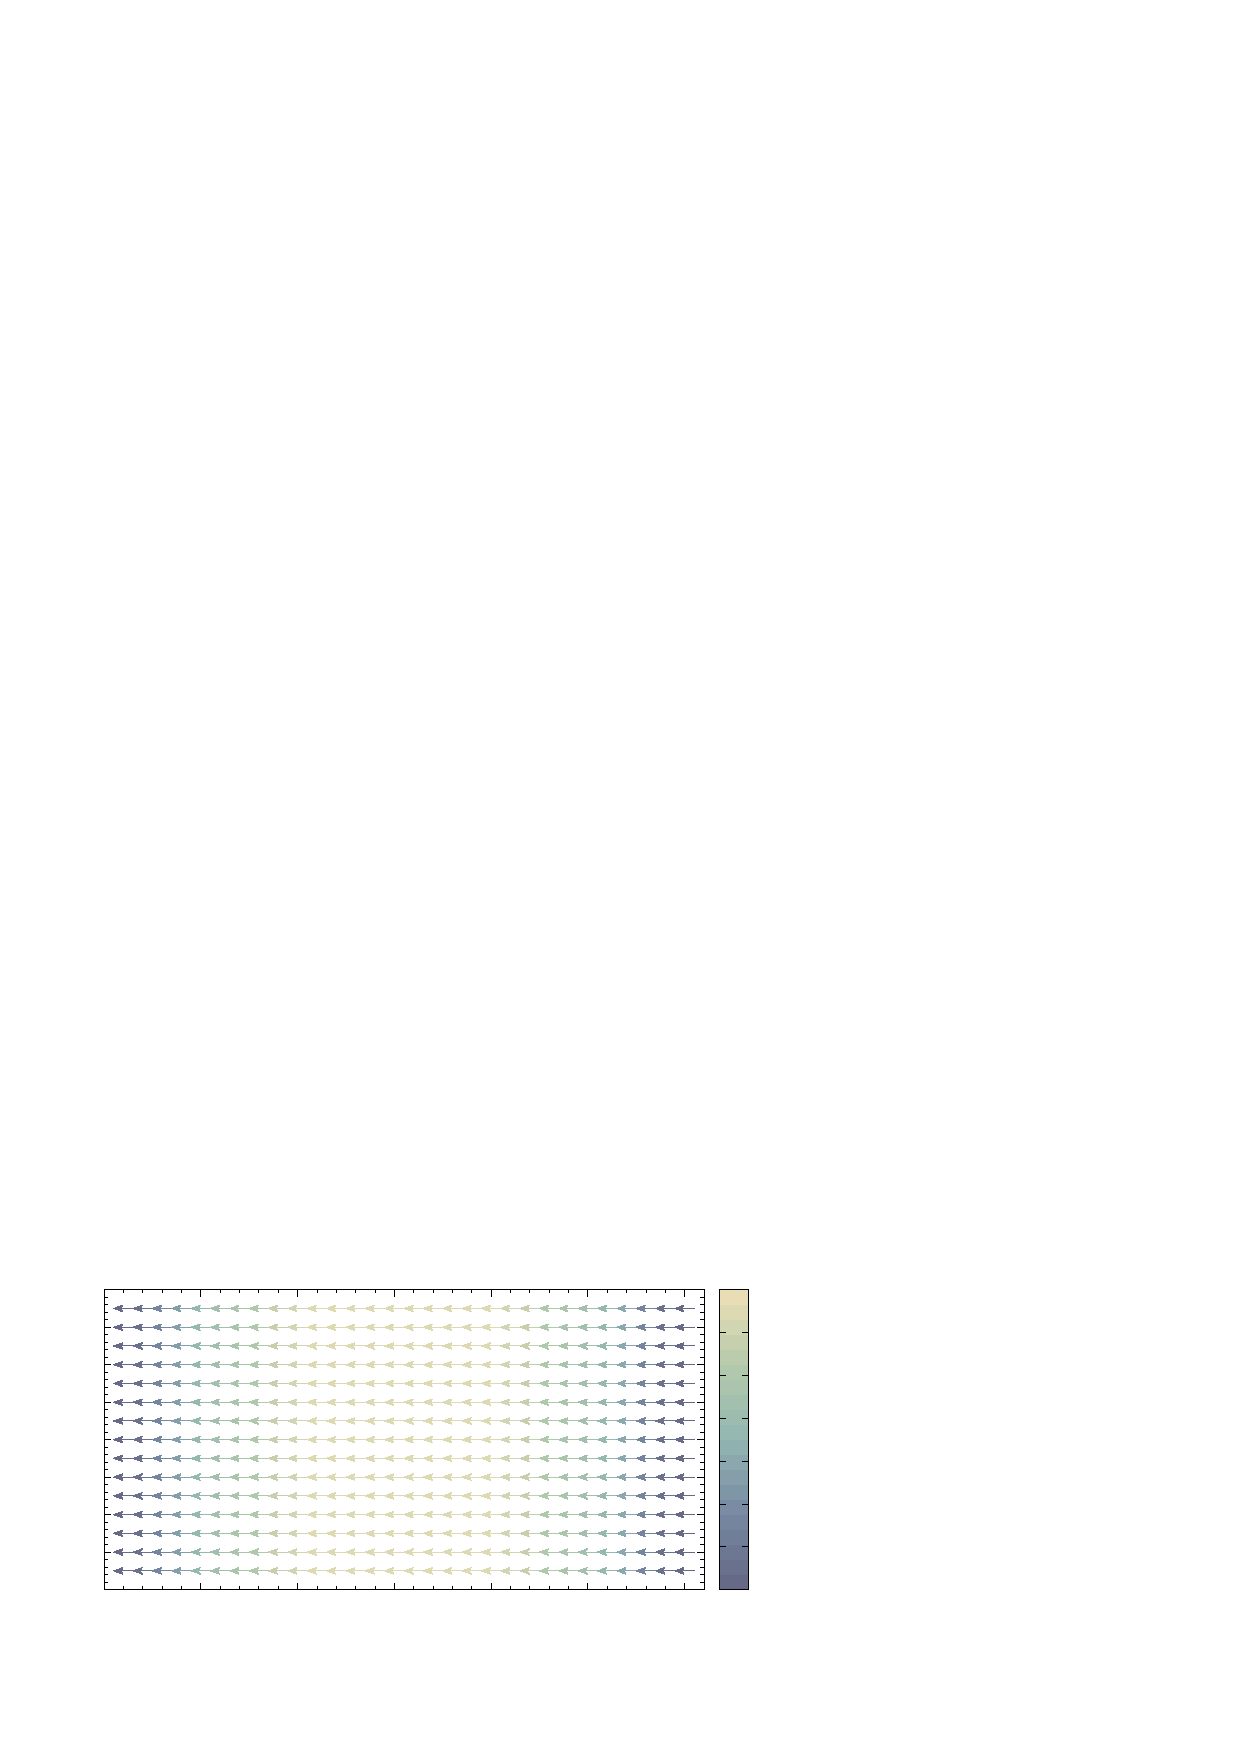
\includegraphics[width={288.00bp},height={188.60bp}]{Plots/SC10AM10/HeatMap/VertHorizBC/plot}}%
    \gplfronttext
  \end{picture}%
\endgroup


    \caption{$\mu = -2.5$}
\end{figure}
\begin{figure}[H]
    \centering
    % GNUPLOT: LaTeX picture with Postscript
\begingroup
  % Encoding inside the plot.  In the header of your document, this encoding
  % should to defined, e.g., by using
  % \usepackage[cp1252,<other encodings>]{inputenc}
  \inputencoding{cp1252}%
  \makeatletter
  \providecommand\color[2][]{%
    \GenericError{(gnuplot) \space\space\space\@spaces}{%
      Package color not loaded in conjunction with
      terminal option `colourtext'%
    }{See the gnuplot documentation for explanation.%
    }{Either use 'blacktext' in gnuplot or load the package
      color.sty in LaTeX.}%
    \renewcommand\color[2][]{}%
  }%
  \providecommand\includegraphics[2][]{%
    \GenericError{(gnuplot) \space\space\space\@spaces}{%
      Package graphicx or graphics not loaded%
    }{See the gnuplot documentation for explanation.%
    }{The gnuplot epslatex terminal needs graphicx.sty or graphics.sty.}%
    \renewcommand\includegraphics[2][]{}%
  }%
  \providecommand\rotatebox[2]{#2}%
  \@ifundefined{ifGPcolor}{%
    \newif\ifGPcolor
    \GPcolortrue
  }{}%
  \@ifundefined{ifGPblacktext}{%
    \newif\ifGPblacktext
    \GPblacktextfalse
  }{}%
  % define a \g@addto@macro without @ in the name:
  \let\gplgaddtomacro\g@addto@macro
  % define empty templates for all commands taking text:
  \gdef\gplbacktext{}%
  \gdef\gplfronttext{}%
  \makeatother
  \ifGPblacktext
    % no textcolor at all
    \def\colorrgb#1{}%
    \def\colorgray#1{}%
  \else
    % gray or color?
    \ifGPcolor
      \def\colorrgb#1{\color[rgb]{#1}}%
      \def\colorgray#1{\color[gray]{#1}}%
      \expandafter\def\csname LTw\endcsname{\color{white}}%
      \expandafter\def\csname LTb\endcsname{\color{black}}%
      \expandafter\def\csname LTa\endcsname{\color{black}}%
      \expandafter\def\csname LT0\endcsname{\color[rgb]{1,0,0}}%
      \expandafter\def\csname LT1\endcsname{\color[rgb]{0,1,0}}%
      \expandafter\def\csname LT2\endcsname{\color[rgb]{0,0,1}}%
      \expandafter\def\csname LT3\endcsname{\color[rgb]{1,0,1}}%
      \expandafter\def\csname LT4\endcsname{\color[rgb]{0,1,1}}%
      \expandafter\def\csname LT5\endcsname{\color[rgb]{1,1,0}}%
      \expandafter\def\csname LT6\endcsname{\color[rgb]{0,0,0}}%
      \expandafter\def\csname LT7\endcsname{\color[rgb]{1,0.3,0}}%
      \expandafter\def\csname LT8\endcsname{\color[rgb]{0.5,0.5,0.5}}%
    \else
      % gray
      \def\colorrgb#1{\color{black}}%
      \def\colorgray#1{\color[gray]{#1}}%
      \expandafter\def\csname LTw\endcsname{\color{white}}%
      \expandafter\def\csname LTb\endcsname{\color{black}}%
      \expandafter\def\csname LTa\endcsname{\color{black}}%
      \expandafter\def\csname LT0\endcsname{\color{black}}%
      \expandafter\def\csname LT1\endcsname{\color{black}}%
      \expandafter\def\csname LT2\endcsname{\color{black}}%
      \expandafter\def\csname LT3\endcsname{\color{black}}%
      \expandafter\def\csname LT4\endcsname{\color{black}}%
      \expandafter\def\csname LT5\endcsname{\color{black}}%
      \expandafter\def\csname LT6\endcsname{\color{black}}%
      \expandafter\def\csname LT7\endcsname{\color{black}}%
      \expandafter\def\csname LT8\endcsname{\color{black}}%
    \fi
  \fi
    \setlength{\unitlength}{0.0500bp}%
    \ifx\gptboxheight\undefined%
      \newlength{\gptboxheight}%
      \newlength{\gptboxwidth}%
      \newsavebox{\gptboxtext}%
    \fi%
    \setlength{\fboxrule}{0.5pt}%
    \setlength{\fboxsep}{1pt}%
    \definecolor{tbcol}{rgb}{1,1,1}%
\begin{picture}(5760.00,3772.00)%
    \gplgaddtomacro\gplbacktext{%
      \csname LTb\endcsname%%
      \put(1807,3313){\makebox(0,0){\strut{}SC}}%
      \put(3953,3313){\makebox(0,0){\strut{}AM}}%
    }%
    \gplgaddtomacro\gplfronttext{%
      \csname LTb\endcsname%%
      \put(1073,742){\makebox(0,0){\scriptsize 2}}%
      \put(1525,742){\makebox(0,0){\scriptsize 4}}%
      \put(1977,742){\makebox(0,0){\scriptsize 6}}%
      \put(2429,742){\makebox(0,0){\scriptsize 8}}%
      \put(2880,742){\makebox(0,0){\scriptsize 10}}%
      \put(3331,742){\makebox(0,0){\scriptsize 12}}%
      \put(3783,742){\makebox(0,0){\scriptsize 14}}%
      \put(4235,742){\makebox(0,0){\scriptsize 16}}%
      \put(4687,742){\makebox(0,0){\scriptsize 18}}%
      \put(2880,478){\makebox(0,0){\small\textbf{Lattice site $i_x$ in $\bm{e}_x$}}}%
      \put(480,1006){\makebox(0,0){\scriptsize 2}}%
      \put(480,1254){\makebox(0,0){\scriptsize 4}}%
      \put(480,1501){\makebox(0,0){\scriptsize 6}}%
      \put(480,1749){\makebox(0,0){\scriptsize 8}}%
      \put(480,1996){\makebox(0,0){\scriptsize 10}}%
      \put(480,2243){\makebox(0,0){\scriptsize 12}}%
      \put(480,2491){\makebox(0,0){\scriptsize 14}}%
      \put(480,2738){\makebox(0,0){\scriptsize 16}}%
      \put(480,2986){\makebox(0,0){\scriptsize 18}}%
      \put(150,1996){\rotatebox{-270.00}{\makebox(0,0){\small\textbf{Lattice site $i_y$ in $\bm{e}_y$}}}}%
      \put(5743,820){\makebox(0,0){\tiny \(0\)}}%
      \put(5743,1212){\makebox(0,0){\tiny \(1e{-06}\)}}%
      \put(5743,1604){\makebox(0,0){\tiny \(2e{-06}\)}}%
      \put(5743,1996){\makebox(0,0){\tiny \(3e{-06}\)}}%
      \put(5743,2388){\makebox(0,0){\tiny \(4e{-06}\)}}%
      \put(5743,2780){\makebox(0,0){\tiny \(5e{-06}\)}}%
      \put(5743,3171){\makebox(0,0){\tiny \(6e{-06}\)}}%
    }%
    \gplbacktext
    \put(0,0){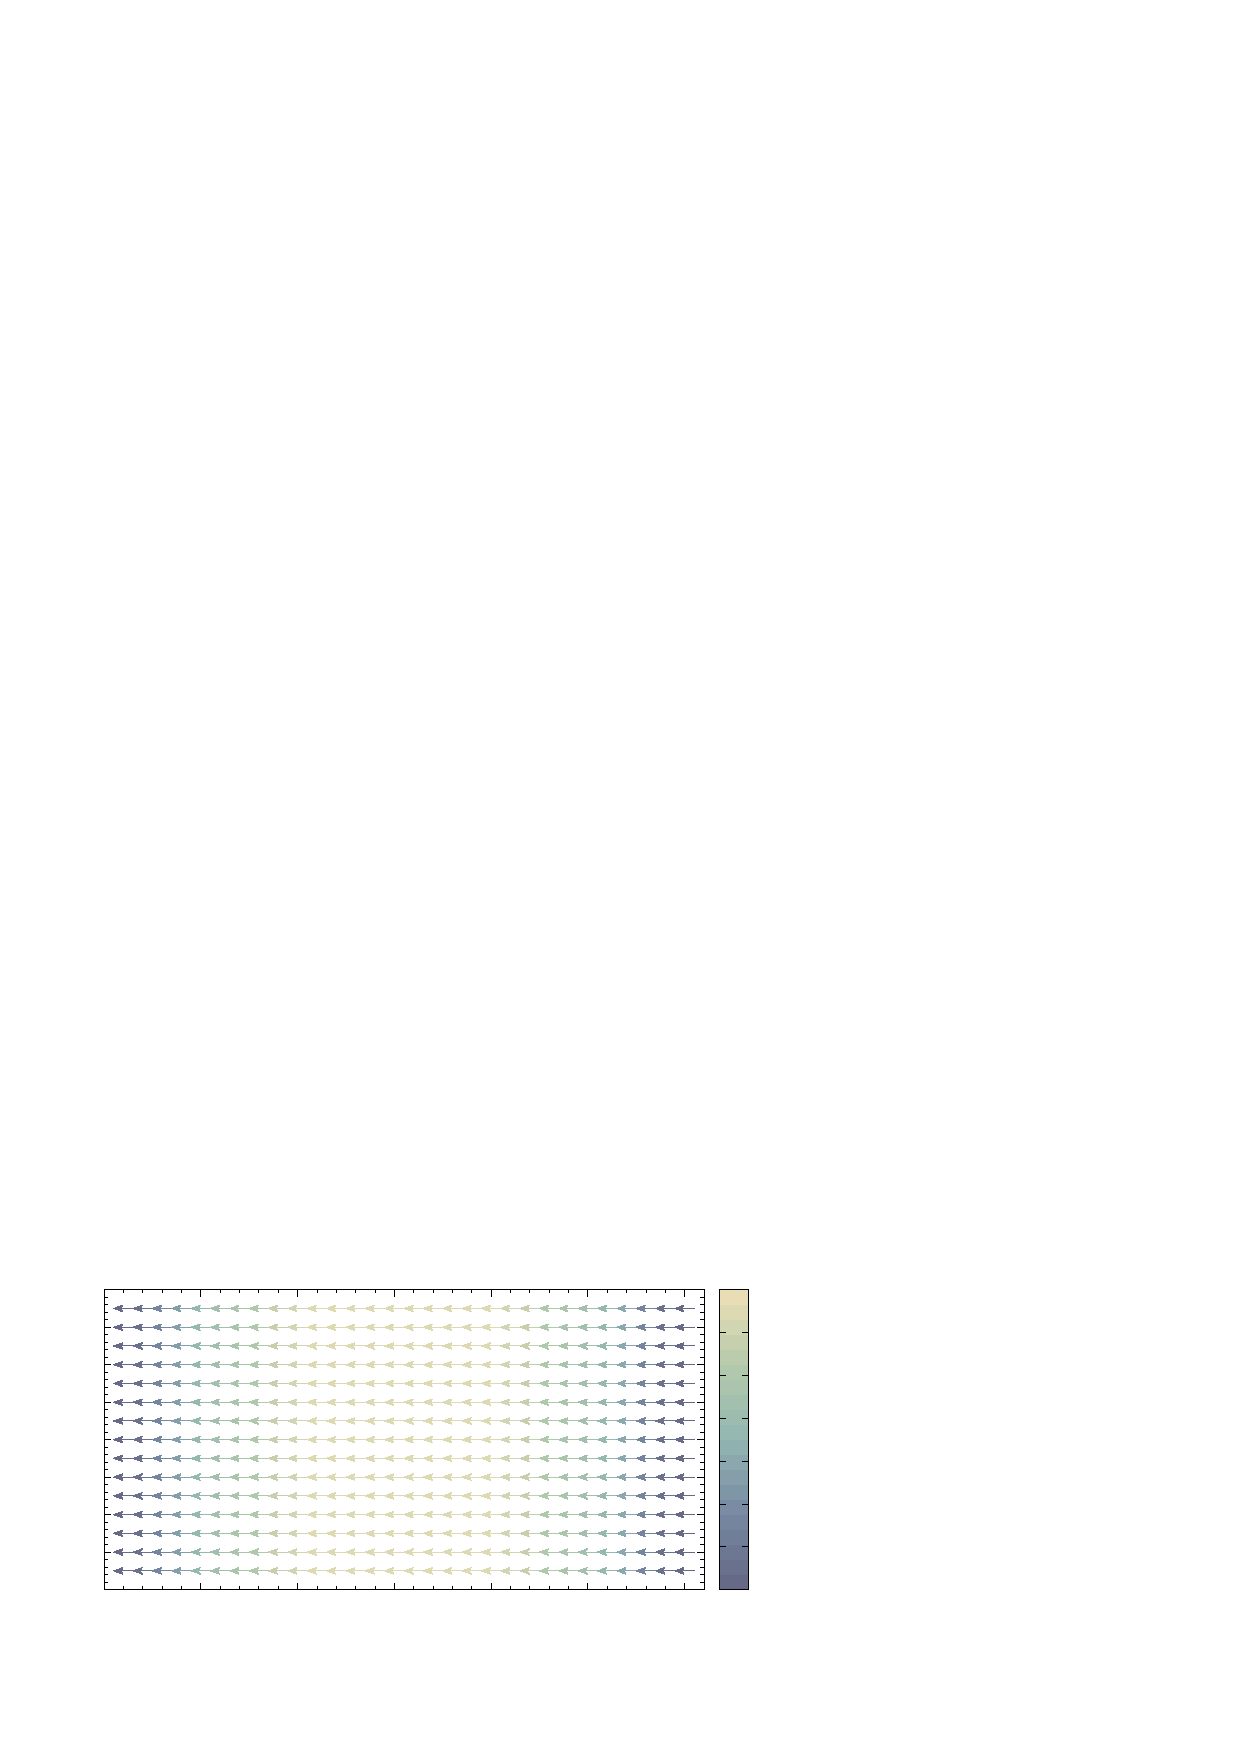
\includegraphics[width={288.00bp},height={188.60bp}]{Plots/SC10AM10/HeatMap/VertHorizBC/plot}}%
    \gplfronttext
  \end{picture}%
\endgroup


    \caption{$\mu = -1.5$}
\end{figure}
\begin{figure}[H]
    \centering
    % GNUPLOT: LaTeX picture with Postscript
\begingroup
  % Encoding inside the plot.  In the header of your document, this encoding
  % should to defined, e.g., by using
  % \usepackage[cp1252,<other encodings>]{inputenc}
  \inputencoding{cp1252}%
  \makeatletter
  \providecommand\color[2][]{%
    \GenericError{(gnuplot) \space\space\space\@spaces}{%
      Package color not loaded in conjunction with
      terminal option `colourtext'%
    }{See the gnuplot documentation for explanation.%
    }{Either use 'blacktext' in gnuplot or load the package
      color.sty in LaTeX.}%
    \renewcommand\color[2][]{}%
  }%
  \providecommand\includegraphics[2][]{%
    \GenericError{(gnuplot) \space\space\space\@spaces}{%
      Package graphicx or graphics not loaded%
    }{See the gnuplot documentation for explanation.%
    }{The gnuplot epslatex terminal needs graphicx.sty or graphics.sty.}%
    \renewcommand\includegraphics[2][]{}%
  }%
  \providecommand\rotatebox[2]{#2}%
  \@ifundefined{ifGPcolor}{%
    \newif\ifGPcolor
    \GPcolortrue
  }{}%
  \@ifundefined{ifGPblacktext}{%
    \newif\ifGPblacktext
    \GPblacktextfalse
  }{}%
  % define a \g@addto@macro without @ in the name:
  \let\gplgaddtomacro\g@addto@macro
  % define empty templates for all commands taking text:
  \gdef\gplbacktext{}%
  \gdef\gplfronttext{}%
  \makeatother
  \ifGPblacktext
    % no textcolor at all
    \def\colorrgb#1{}%
    \def\colorgray#1{}%
  \else
    % gray or color?
    \ifGPcolor
      \def\colorrgb#1{\color[rgb]{#1}}%
      \def\colorgray#1{\color[gray]{#1}}%
      \expandafter\def\csname LTw\endcsname{\color{white}}%
      \expandafter\def\csname LTb\endcsname{\color{black}}%
      \expandafter\def\csname LTa\endcsname{\color{black}}%
      \expandafter\def\csname LT0\endcsname{\color[rgb]{1,0,0}}%
      \expandafter\def\csname LT1\endcsname{\color[rgb]{0,1,0}}%
      \expandafter\def\csname LT2\endcsname{\color[rgb]{0,0,1}}%
      \expandafter\def\csname LT3\endcsname{\color[rgb]{1,0,1}}%
      \expandafter\def\csname LT4\endcsname{\color[rgb]{0,1,1}}%
      \expandafter\def\csname LT5\endcsname{\color[rgb]{1,1,0}}%
      \expandafter\def\csname LT6\endcsname{\color[rgb]{0,0,0}}%
      \expandafter\def\csname LT7\endcsname{\color[rgb]{1,0.3,0}}%
      \expandafter\def\csname LT8\endcsname{\color[rgb]{0.5,0.5,0.5}}%
    \else
      % gray
      \def\colorrgb#1{\color{black}}%
      \def\colorgray#1{\color[gray]{#1}}%
      \expandafter\def\csname LTw\endcsname{\color{white}}%
      \expandafter\def\csname LTb\endcsname{\color{black}}%
      \expandafter\def\csname LTa\endcsname{\color{black}}%
      \expandafter\def\csname LT0\endcsname{\color{black}}%
      \expandafter\def\csname LT1\endcsname{\color{black}}%
      \expandafter\def\csname LT2\endcsname{\color{black}}%
      \expandafter\def\csname LT3\endcsname{\color{black}}%
      \expandafter\def\csname LT4\endcsname{\color{black}}%
      \expandafter\def\csname LT5\endcsname{\color{black}}%
      \expandafter\def\csname LT6\endcsname{\color{black}}%
      \expandafter\def\csname LT7\endcsname{\color{black}}%
      \expandafter\def\csname LT8\endcsname{\color{black}}%
    \fi
  \fi
    \setlength{\unitlength}{0.0500bp}%
    \ifx\gptboxheight\undefined%
      \newlength{\gptboxheight}%
      \newlength{\gptboxwidth}%
      \newsavebox{\gptboxtext}%
    \fi%
    \setlength{\fboxrule}{0.5pt}%
    \setlength{\fboxsep}{1pt}%
    \definecolor{tbcol}{rgb}{1,1,1}%
\begin{picture}(5760.00,3772.00)%
    \gplgaddtomacro\gplbacktext{%
      \csname LTb\endcsname%%
      \put(1807,3313){\makebox(0,0){\strut{}SC}}%
      \put(3953,3313){\makebox(0,0){\strut{}AM}}%
    }%
    \gplgaddtomacro\gplfronttext{%
      \csname LTb\endcsname%%
      \put(1073,742){\makebox(0,0){\scriptsize 2}}%
      \put(1525,742){\makebox(0,0){\scriptsize 4}}%
      \put(1977,742){\makebox(0,0){\scriptsize 6}}%
      \put(2429,742){\makebox(0,0){\scriptsize 8}}%
      \put(2880,742){\makebox(0,0){\scriptsize 10}}%
      \put(3331,742){\makebox(0,0){\scriptsize 12}}%
      \put(3783,742){\makebox(0,0){\scriptsize 14}}%
      \put(4235,742){\makebox(0,0){\scriptsize 16}}%
      \put(4687,742){\makebox(0,0){\scriptsize 18}}%
      \put(2880,478){\makebox(0,0){\small\textbf{Lattice site $i_x$ in $\bm{e}_x$}}}%
      \put(480,1006){\makebox(0,0){\scriptsize 2}}%
      \put(480,1254){\makebox(0,0){\scriptsize 4}}%
      \put(480,1501){\makebox(0,0){\scriptsize 6}}%
      \put(480,1749){\makebox(0,0){\scriptsize 8}}%
      \put(480,1996){\makebox(0,0){\scriptsize 10}}%
      \put(480,2243){\makebox(0,0){\scriptsize 12}}%
      \put(480,2491){\makebox(0,0){\scriptsize 14}}%
      \put(480,2738){\makebox(0,0){\scriptsize 16}}%
      \put(480,2986){\makebox(0,0){\scriptsize 18}}%
      \put(150,1996){\rotatebox{-270.00}{\makebox(0,0){\small\textbf{Lattice site $i_y$ in $\bm{e}_y$}}}}%
      \put(5743,820){\makebox(0,0){\tiny \(0\)}}%
      \put(5743,1212){\makebox(0,0){\tiny \(1e{-06}\)}}%
      \put(5743,1604){\makebox(0,0){\tiny \(2e{-06}\)}}%
      \put(5743,1996){\makebox(0,0){\tiny \(3e{-06}\)}}%
      \put(5743,2388){\makebox(0,0){\tiny \(4e{-06}\)}}%
      \put(5743,2780){\makebox(0,0){\tiny \(5e{-06}\)}}%
      \put(5743,3171){\makebox(0,0){\tiny \(6e{-06}\)}}%
    }%
    \gplbacktext
    \put(0,0){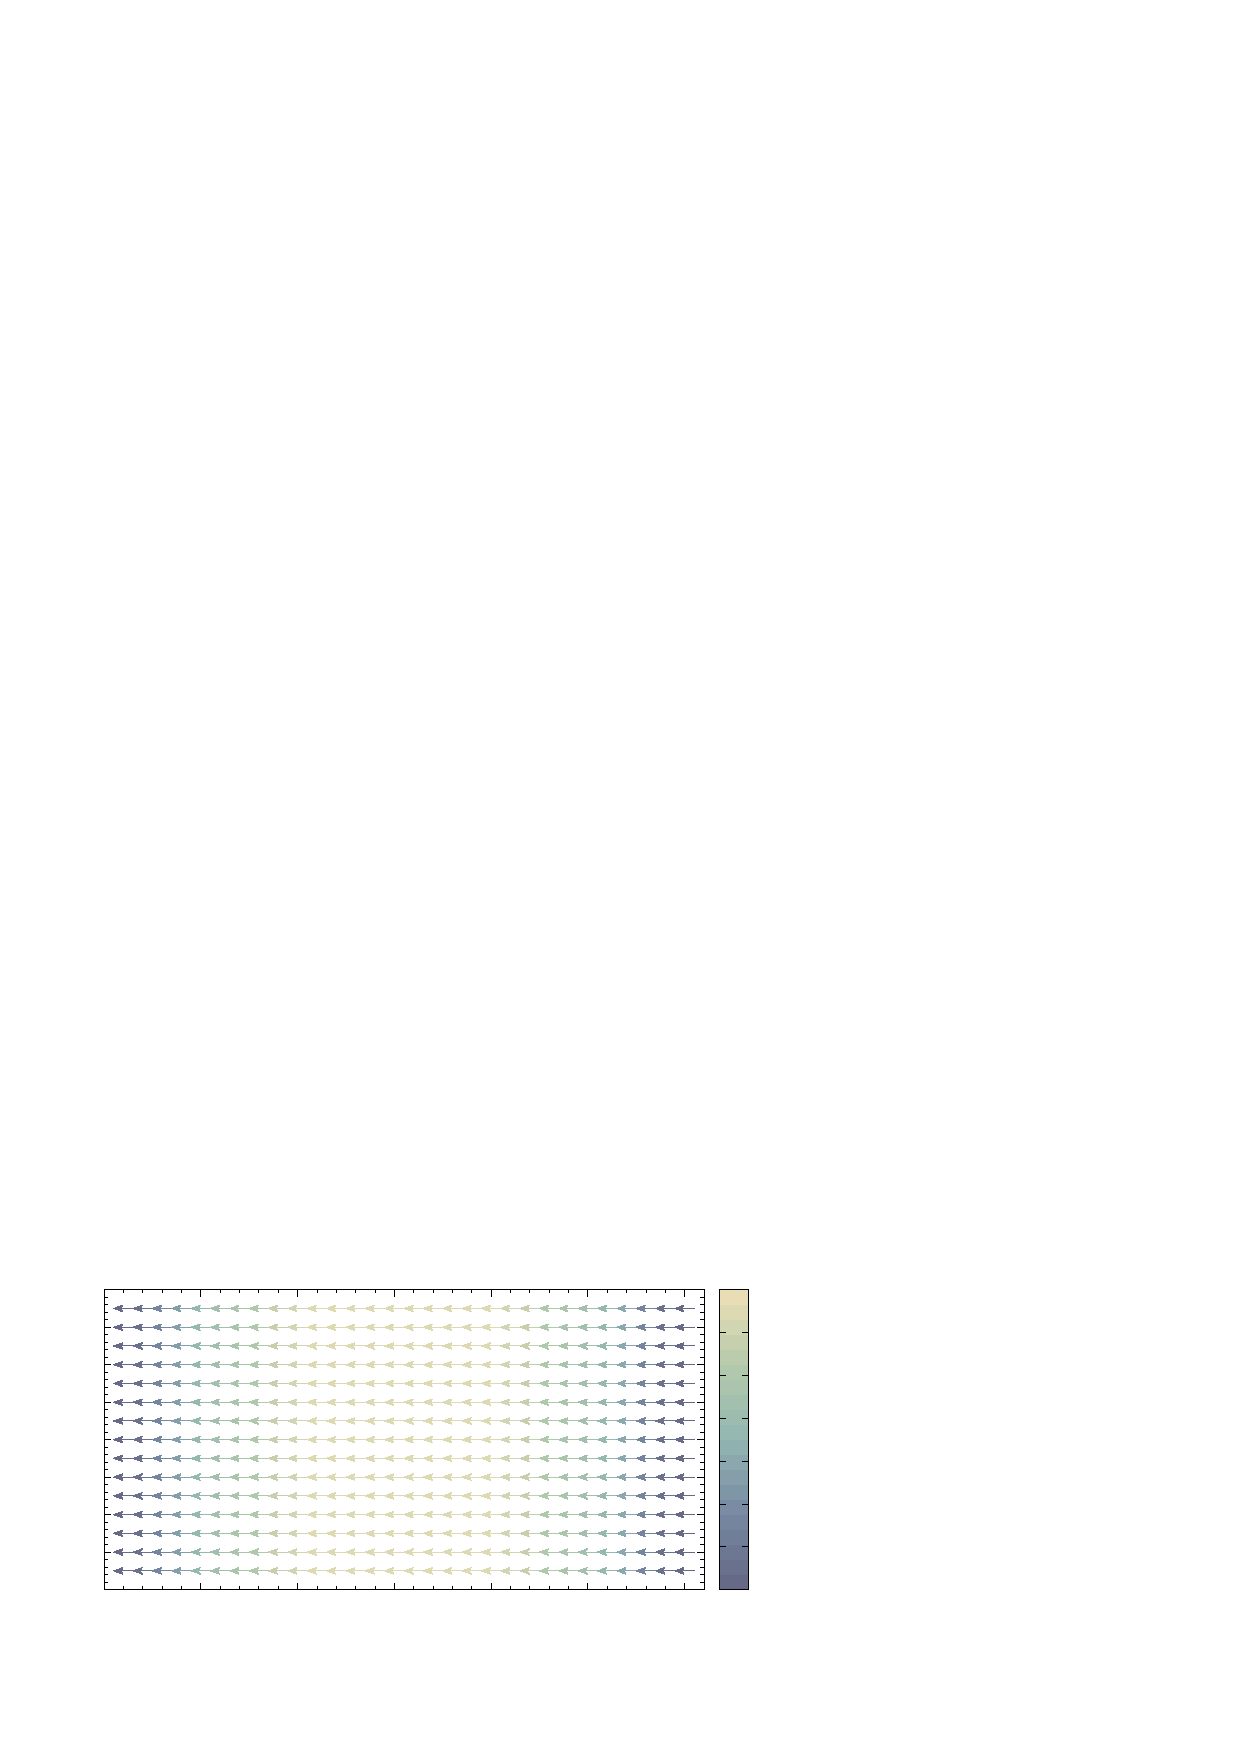
\includegraphics[width={288.00bp},height={188.60bp}]{Plots/SC10AM10/HeatMap/VertHorizBC/plot}}%
    \gplfronttext
  \end{picture}%
\endgroup


    \caption{$\mu = -0.5$}
\end{figure}
The superconductivity fills uniformaly the superconductor. It's magnetude seams to grow with while $|\mu|$ get closer to zero.
Once again the oscillating exponential decay is present. We count up to eight oscillations for the three cases of study, whose
frequency is arround three sites in all configurations. The oscillations takes only place along the $x$ axis but the exponential decay
seams to point along the normal of the interface, making the (40,0) region the less populated in Cooper pairs.
The lower the $|\mu|$, the less noise we observe in the plots. Similarly to the straight interface the decay is strong in the begging
and then slows down when approching the farest regions from the interface.\\


% \begin{tikzpicture}
%     \begin{axis}[
%         view={0}{90},  % Adjust the viewing angle
%         axis lines=center,
%         xlabel={$x$}, ylabel={$y$}, zlabel={$z$},
%         domain=-2*pi:2*pi, domain y=-2*pi:2*pi,
%         colormap/cool,
%       ]
%       % \addplot3[
%       %   surf,
%       %   shader=flat,
%       %   samples=50,
%       %   samples y=50,
%       %   z buffer=sort,
%       %   unbounded coords=jump,
%       % ]
%       % ({fd(x)},{y},{fd(x)}); % Using fd(x) for z-value

%       \addplot3[
%         surf,
%         shader=flat,
%         samples=100,
%         samples y=100,
%         z buffer=sort,
%         unbounded coords=jump,
%       ]
%       ({x},{y},{f(x,y,2)}); % Change th{f(x,y,0.5)}e last parameter (2) to set "a" \pgfmathifthenelse{abs(cos(x-pi) + cos(y-pi) - 2/2) < 1e-3}{2}{-2}}
%     \end{axis}
%   \end{tikzpicture}
\rem{A side view to comapre the oscilaltion amplitude.}

In the same way than before, this increase in Cooper pairs formation with degrowing $|\mu|$ is due to the shape of the fermi surface.
For $\mu=-2.5$ we see that the populated region do not especialy fully fill the states occuped by the s-wave. 
For $\mu=-1.5$ the populated region is larger more states can be found in the s-wave. 
For $\mu=-0.5$ we oberve a factor two increase in the number of Cooper pairs, while we have a factor ten between the first two cases.
This is most likely due to the fact that the fermi surface at $\mu=-1.5$ was already very close to the shape of the s-wave in the momentum space.
Therfore the majority of the newly accessible states are outside the s-wave range,
resulting in a smaller increase in the number of Cooper pairs when compared to the case of $\mu=-2.5$.



\end{document}